\section{Model Architecture}
\label{sec:scale_asr:model}

A simple multi-layer model with a single recurrent layer cannot exploit
thousands of hours of labelled speech. In order to learn from datasets this
large, we increase the model capacity via depth. We explore architectures with
up to 11 layers including many bidirectional recurrent layers and convolutional
layers. These models have nearly 8 times the amount of computation per data
example as the models in Deep Speech 1 making fast optimization and computation
critical. In order to optimize these models successfully, we use Batch
Normalization for RNNs and a novel optimization curriculum we call SortaGrad.
We also exploit long \emph{strides} between RNN inputs to reduce computation
per example by a factor of 3. This is helpful for both training and evaluation,
though requires some modifications in order to work well with CTC. Finally,
though many of our research results make use of bidirectional recurrent layers,
we find that excellent models exist using only unidirectional recurrent
layers---a feature that makes such models much easier to deploy.  Taken
together these features allow us to tractably optimize deep RNNs and improve
performance by more than 40\% in both English and Mandarin error rates over the
smaller baseline models.

\subsection{Preliminaries}

Figure~\ref{fig:scaling_asr:ds2_network} shows the architecture of the DS2
system which at its core is similar to the previous DS1
system~\cite{hannun2014deepspeech}: a recurrent neural network (RNN) trained to
ingest speech spectrograms and generate text transcriptions. 

Let a single utterance $x^{(i)}$ and label $y^{(i)}$ be sampled from a training
set $\mathcal{X} = \{(x^{(1)},y^{(1)}),(x^{(2)},y^{(2)}),\ldots\}$. Each
utterance, $x^{(i)}$, is a time-series of length $T^{(i)}$ where every
time-slice is a vector of audio features, $x_t^{(i)},  t=0,\ldots,T^{(i)}-1$.
We use a spectrogram of power normalized audio clips as the features to the
system, so $x^{(i)}_{t,p}$ denotes the power of the $p$'th frequency bin in the
audio frame at time $t$. The goal of the RNN is to convert an input sequence
$x^{(i)}$ into a final transcription $y^{(i)}$. For notational convenience, we
drop the superscripts and use $x$ to denote a chosen utterance and $y$ the
corresponding label.

The outputs of the network are the graphemes of each language. At each output
time-step $t$, the RNN makes a prediction over characters, $p(\ell_t | x)$,
where $\ell_t$ is either a character in the alphabet or the blank symbol. In
English we have $\ell_t \in \{\textrm{a, b, c, }\ldots, \textrm{z},
\textit{space}, \textit{apostrophe}, \textit{blank}\}$, where we have added the
\textit{apostrophe} as well as a \textit{space} symbol to denote word
boundaries. For the Mandarin system the network outputs simplified Chinese
characters.  We describe this in more detail in
Section~\ref{sec:scaling_asr:chinesemodel}.

\begin{figure}
    \centering
    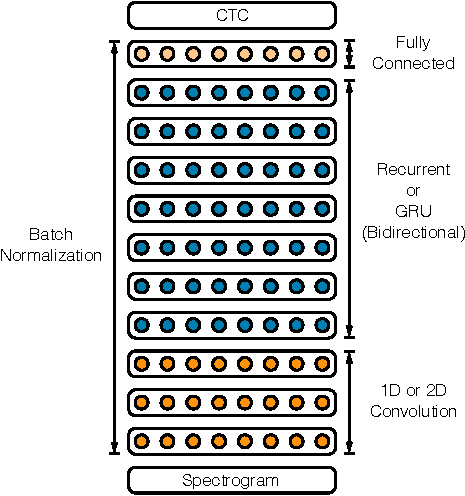
\includegraphics[width=0.6\textwidth]{scaling_asr/figures/ds2_architecture.pdf}
    \caption{The architecture of the DS2 network used for both English and
             Mandarin speech.}
    \label{fig:scaling_asr:ds2_network}
\end{figure}

The RNN model is composed of several layers of hidden units. The architectures
we experiment with consist of one or more convolutional layers, followed by one
or more recurrent layers, followed by one or more fully connected layers.

The hidden representation at layer $l$ is given by $h^l$ with the convention
that $h^0$ represents the input $x$. The bottom of the network is one or more
convolutions over the time dimension of the input. For a context window of size
$c$, the $i$-th activation at time-step $t$ of the convolutional layer is given
by
\begin{equation*}
h_{t,i}^l = f( w_i^l \circ h^{l-1}_{t-c:t+c} )
\end{equation*}
where $\circ$ denotes the element-wise product between the $i$-th filter and
the context window of the previous layers activations, and $f$ denotes a unary
nonlinear function. We use the clipped rectified-linear (ReLU) function $f(x) =
\min\{\max\{x, 0\},20\}$ as our nonlinearity. In some layers, usually the
first, we sub-sample by striding the convolution by $s$ frames. The goal is to
shorten the number of time-steps for the recurrent layers above.

Following the convolutional layers are one or more bidirectional recurrent
layers~\cite{schuster1997bidirectional}. The forward in time
$\overrightarrow{h}^l$ and backward in time $\overleftarrow{h}^l$ recurrent
layer activations are computed as
\begin{equation*}
\begin{aligned}
    \overrightarrow{h}_t^l &= g( h_t^{l-1}, \overrightarrow{h}_{t-1}^l ) \\
    \overleftarrow{h}_t^l &= g( h_t^{l-1}, \overleftarrow{h}_{t+1}^l )
\end{aligned}
\end{equation*}
The two sets of activations are summed to form the output activations for the
layer $h^l = \overrightarrow{h}^l + \overleftarrow{h}^l$.  The function
$g(\cdot)$ can be the standard recurrent operation
\begin{equation}
    \overrightarrow{h}_t^l = g( h_t^{l-1}, \overrightarrow{h}_{t-1}^l )
        = f( W^l h_t^{l-1} + \overrightarrow{U}^l \overrightarrow{h}_{t-1}^l + b^l )
    \label{eq:scaling_asr:plainrnn}
\end{equation}
where $W^l$ is the input-hidden weight matrix, $\overrightarrow{U}^l$ is the
recurrent weight matrix and $b^l$ is a bias term. In this case the input-hidden
weights are shared for both directions of the recurrence. The function
$g(\cdot)$ can also represent more complex recurrence operations such as the
Long Short-Term Memory (LSTM) units~\cite{hochreiter1997} and the gated
recurrent units (GRU)~\cite{cho2014}.

After the bidirectional recurrent layers we apply one or more fully connected layers with
\begin{equation*}
    h^l_t = f( W^l h^{l-1}_t + b^l )
\end{equation*}
The output layer $L$ is a softmax computing a probability distribution over characters given by
\begin{equation*}
    p(\ell_t=k \mid x) = \frac{\exp(w^L_k \cdot h^{L-1}_t)}{\sum_j \exp(w^L_j \cdot h^{L-1}_t)}
\end{equation*}

The model is trained using the CTC loss function~\cite{graves2006}. Given an
input-output pair $(x, y)$ and the current parameters of the network $\theta$,
we compute the loss function $\mathcal{L}(x, y; \theta)$ and its derivative
with respect to the parameters of the network $\nabla_\theta \mathcal{L}(x, y;
\theta)$. This derivative is then used to update the network parameters through
the backpropagation through time algorithm.

In the following subsections we describe the architectural and algorithmic
improvements made relative to DS1~\cite{hannun2014deepspeech}.  Unless
otherwise stated these improvements are language agnostic. We report results on
an English speaker held out development set which is an internal dataset
containing 2048 utterances of primarily read speech. All models are trained on
datasets described in Section~\ref{sec:scaling_asr:data}. We report Word Error
Rate (WER) for the English system and Character Error Rate (CER) for the
Mandarin system. In both cases we integrate a language model in a beam search
decoding step as described in Section~\ref{sec:scaling_asr:languagemodel}.


\subsection{Batch Normalization for Deep RNNs}
\label{sec:scaling_asr:bn}

To efficiently scale our model as we scale the training set, we increase the
depth of the networks by adding more hidden layers, rather than making each
layer larger. Previous work has examined doing so by increasing the number of
consecutive bidirectional recurrent layers~\cite{graves2013}. We explore Batch
Normalization (BatchNorm) as a technique to accelerate training for such
networks~\cite{ioffe2015batch} since they often suffer from optimization
issues. 

Recent research has shown that BatchNorm improves the speed of convergence of
recurrent nets, without showing any improvement in generalization
performance~\cite{laurent2016}. In contrast, we demonstrate that when applied
to very deep networks of simple RNNs on large data sets, batch normalization
substantially improves final generalization error while greatly accelerating
training. 

In a typical feed-forward layer containing an affine transformation followed by
a non-linearity $f(\cdot)$, we insert a BatchNorm transformation by applying
$f(\mathcal{B}(Wh))$ instead of $f(Wh + b)$, where
\begin{equation*}
    \mathcal{B}(x) = \gamma 
        \frac{x - \mathrm{E}[x]}{\left(\mathrm{Var}[x] + \epsilon\right)^{1/2}} + \beta.
\end{equation*}
The terms $\mathrm{E}$ and $\mathrm{Var}$ are the empirical mean and variance
over a minibatch. The bias $b$ of the layer is dropped since its effect is
cancelled by mean removal. The learnable parameters $\gamma$ and $\beta$ allow
the layer to scale and shift each hidden unit as desired. The constant
$\epsilon$ is small and positive, and is included only for numerical stability.
In our convolutional layers the mean and variance are estimated over all the
temporal output units for a given convolutional filter on a minibatch. The
BatchNorm transformation reduces \emph{internal covariate shift} by insulating
a given layer from potentially uninteresting changes in the mean and variance
of the layer's input.

We consider two methods of extending BatchNorm to bidirectional
RNNs~\cite{laurent2016}. A natural extension is to insert a BatchNorm
transformation immediately before every non-linearity.
Equation~\ref{eq:scaling_asr:plainrnn} then becomes 
\begin{equation*}
    \overrightarrow{h}^l_t =
        f( \mathcal{B}( W^l h^{l-1}_t + \overrightarrow{U}^l \overrightarrow{h}^l_{t-1} )).  
\end{equation*}
In this case the mean and variance statistics are accumulated over a single
time-step of the minibatch. The sequential dependence between time-steps
prevents averaging over all time-steps. We find that this technique does not
lead to improvements in optimization. We also tried accumulating an average
over successive time-steps, so later time-steps are normalized over all present
and previous time-steps. This also proved ineffective and greatly complicated
backpropagation.

We find that \emph{sequence-wise} normalization~\cite{laurent2016} overcomes
these issues. The recurrent computation is given by
\begin{equation*}
    \overrightarrow{h}^l_t = f( \mathcal{B}( W^l h^{l-1}_t) + \overrightarrow{U}^l \overrightarrow{h}^l_{t-1}).  
\end{equation*}

\begin{table}
\centering
\begin{tabular}{l  c  r r r  r  r r r  r}
\toprule
Architecture & Hidden Units & \multicolumn{4}{c}{Train} & \multicolumn{4}{c}{Dev}  \\
\midrule
     &  & \multicolumn{3}{c}{Baseline} & BatchNorm & \multicolumn{3}{c}{Baseline} & BatchNorm \\
\midrule
1 RNN, 5 total   & 2400 & & 10.55 & & 11.99 & & 13.55 & & 14.40 \\
3 RNN, 5 total   & 1880 & & 9.55  & & 8.29  & & 11.61 & & 10.56 \\
5 RNN, 7 total   & 1510 & & 8.59  & & 7.61  & & 10.77 & & 9.78 \\
7 RNN, 9 total   & 1280 & & 8.76  & & 7.68  & & 10.83 & & 9.52 \\
\bottomrule
\end{tabular}
\caption{Comparison of WER on a training and development set for various depths
         of RNN, with and without BatchNorm. The number of parameters is kept
         constant as the depth increases, thus the number of hidden units per layer
         decreases. All networks have 38 million parameters. The architecture ``M
         RNN, N total'' implies 1 layer of 1D convolution at the input, M
         consecutive bidirectional RNN layers, and the rest as fully-connected
         layers with N total layers in the network.}
\label{table:scaling_asr:batch_norm}
\end{table}

For each hidden unit, we compute the mean and variance statistics over all
items in the minibatch over the length of the sequence.
Figure~\ref{fig:scaling_asr:bn} shows that deep networks converge faster with
sequence-wise normalization.  Table~\ref{table:scaling_asr:batch_norm} shows
that the performance improvement from sequence-wise normalization increases
with the depth of the network, with a 12\% performance difference for the
deepest network. When comparing depth, in order to control for model size we
hold constant the total number of parameters and still see strong performance
gains. We would expect to see even larger improvements from depth if we held
constant the number of activations per layer and added layers. We also find
that BatchNorm harms generalization error for the shallowest network just as it
converges slower for shallower networks. 

The BatchNorm approach works well in training, but is difficult to implement
for a deployed ASR system, since it is often necessary to evaluate a single
utterance in deployment rather than a batch. We find that normalizing each
neuron to its mean and variance over just the sequence degrades performance.
Instead, we store a running average of the mean and variance for the neuron
collected during training, and use these for evaluation in
deployment~\cite{ioffe2015batch}. Using this technique, we can evaluate a
single utterance at a time with better results than evaluating with a large
batch.

\begin{figure}
\centering
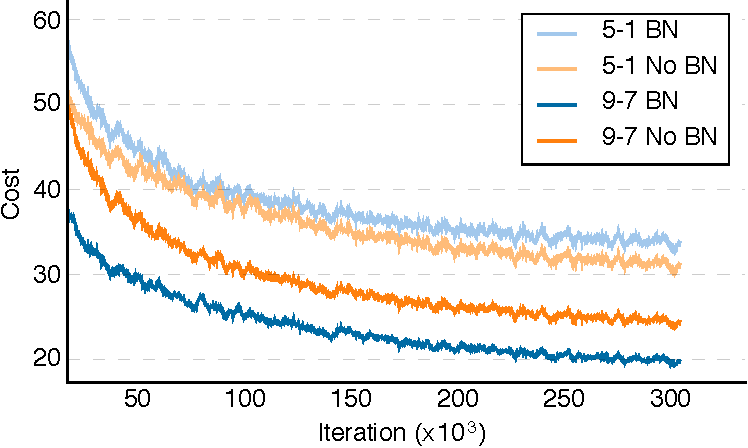
\includegraphics[width=0.6\textwidth]{scaling_asr/figures/bn_nobn.pdf}
\caption{Training curves of two models trained with and without BatchNorm. We
         start the plot after the first epoch of training as the curve is more
         difficult to interpret due to the SortaGrad curriculum.}
\label{fig:scaling_asr:bn}
\end{figure}

\subsection{SortaGrad}

Training on examples of varying length pose some algorithmic challenges. One
possible solution is truncating backpropagation through
time~\cite{williams1990}, so that all examples have the same sequence length
during training~\cite{sainath2015}. However, this can inhibit the ability to
learn longer term dependencies. Other works have found that presenting examples
in order of difficulty can accelerate online
learning~\cite{bengio2009curriculum, zaremba2014}. A common theme in many
sequence learning problems including machine translation and speech recognition
is that longer examples tend to be more challenging~\cite{cho2014}.

The CTC cost function that we use implicitly depends on the length of the
utterance,
\begin{equation}
\label{eq:scaling_asr:ctc}
    \mathcal{L}(x, y; \theta) = -\log \sum_{\ell \in \textrm{Align}(x, y)}
        \prod_t^{T} p_{\textrm{ctc}}(\ell_t \mid x; \theta).
\end{equation}
where $\textrm{Align}(x, y)$ is the set of all possible alignments of the
characters of the transcription $y$ to frames of input $x$ under the CTC
operator. In equation~\ref{eq:scaling_asr:ctc}, the inner term is a product
over time-steps of the sequence, which shrinks with the length of the sequence
since $p_{\textrm{ctc}}(\ell_t \mid x;\theta)<1$. This motivates a curriculum
learning strategy we title SortaGrad. SortaGrad uses the length of the
utterance as a heuristic for difficulty, since long utterances have higher cost
than short utterances.

\begin{table}
\centering
\begin{tabular}{l  r r r  r  r r r  r}
\toprule
& \multicolumn{4}{c}{Train} & \multicolumn{4}{c}{Dev}\\
\midrule
& \multicolumn{3}{c}{Baseline} &  BatchNorm & \multicolumn{3}{c}{Baseline} & BatchNorm\\
\midrule
Not Sorted & & 10.71 & & 8.04 & & 11.96 & & 9.78 \\
Sorted     & & 8.76 & & 7.68 & & 10.83 & & 9.52 \\
\bottomrule
\end{tabular}
\caption{Comparison of WER on a training and development set with and without
         SortaGrad, and with and without BatchNorm.}
\label{table:scaling_asr:sorting}
\end{table}

In the first training epoch, we iterate through the training set in increasing
order of the length of the longest utterance in the minibatch. After the first
epoch, training reverts back to a random order over minibatches.
Table~\ref{table:scaling_asr:sorting} shows a comparison of training cost with
and without SortaGrad on the 9 layer model with 7 recurrent layers. This effect
is particularly pronounced for networks without BatchNorm, since they are
numerically less stable. In some sense the two techniques substitute for one
another, though we still find gains when applying SortaGrad and BatchNorm
together. Even with BatchNorm we find that this curriculum improves numerical
stability and sensitivity to small changes in training. Numerical instability
can arise from different transcendental function implementations in the CPU and
the GPU, especially when computing the CTC cost. This curriculum gives
comparable results for both implementations.

We suspect that these benefits occur primarily because long utterances tend to
have larger gradients, yet we use a fixed learning rate independent of
utterance length. Furthermore, longer utterances are more likely to cause the
internal state of the RNNs to explode at an early stage in training.

\subsection{Comparison of simple RNNs and GRUs}

The models we have shown so far are \emph{simple} RNNs that have bidirectional
recurrent layers with the recurrence for both the forward in time and backward
in time directions modeled by Equation~\ref{eq:scaling_asr:plainrnn}. Current
research in speech and language processing has shown that having a more complex
recurrence can allow the network to remember state over more time-steps while
making them more computationally expensive to train~\cite{sainath2015,
chan2016, sutskever2014, bahdanau2016}. Two commonly used recurrent
architectures are the Long Short-Term Memory (LSTM)
units~\cite{hochreiter1997} and the Gated Recurrent Units
(GRU)~\cite{cho2014}, though many other variations exist. A recent
comprehensive study of thousands of variations of LSTM and GRU architectures
showed that a GRU is comparable to an LSTM with a properly initialized forget
gate bias, and their best variants are competitive with each
other~\cite{jozefowicz2015}. We decided to examine GRUs because experiments on
smaller data sets showed the GRU and LSTM reach similar accuracy for the same
number of parameters, but the GRUs were faster to train and less likely to
diverge. 

The GRUs we use are computed by 
\begin{equation*}
\begin{aligned}
z_t &= \sigma(W_z x_t + U_z h_{t-1} + b_z) \\
r_t &= \sigma(W_r x_t + U_r h_{t-1} + b_r) \\
\tilde{h}_t &= f(W_h x_t + r_t \circ U_h h_{t-1} + b_h) \\
h_t &= (1 - z_t) h_{t-1} + z_t \tilde{h}_t
\end{aligned}
\end{equation*}

where $\sigma(\cdot)$ is the sigmoid function, $z$ and $r$ represent the
\emph{update} and \emph{reset} gates respectively, and we drop the layer
superscripts for simplicity. We differ slightly from the standard GRU in that
we multiply the hidden state $h_{t-1}$ by $U_h$ prior to scaling by the reset
gate. This allows for all operations on $h_{t-1}$ to be computed in a single
matrix multiplication. The output nonlinearity $f(\cdot)$ is typically the
hyperbolic tangent function $tanh$. However, we find similar performance for
$tanh$ and clipped-ReLU nonlinearities and choose to use the clipped-ReLU for
simplicity and uniformity with the rest of the network.

\begin{table}
\centering
\begin{tabular}{l  r  r}
\toprule
Architecture &  Simple RNN & GRU \\
\midrule
5 layers, 1 Recurrent   & 14.40 & 10.53  \\
5 layers, 3 Recurrent   & 10.56 & 8.00  \\
7 layers, 5 Recurrent   & 9.78 & 7.79  \\
9 layers, 7 Recurrent   & 9.52 & 8.19  \\
\bottomrule
\end{tabular}
\caption{Comparison of development set WER for networks with either simple RNN
         or GRU, for various depths.}
\label{table:scaling_asr:rnns}
\end{table}

Both GRU and simple RNN architectures benefit from batch normalization and show
strong results with deep networks. However, Table~\ref{table:scaling_asr:rnns}
shows that for a fixed number of parameters, the GRU architectures achieve
better WER for all network depths. This is clear evidence of the long term
dependencies inherent in the speech recognition task present both within
individual words and between words. As we discuss in
Section~\ref{sec:scaling_asr:languagemodel}, even simple RNNs are able to
implicitly learn a language model due to the large amount of training data.
Interestingly, the GRU networks with 5 or more recurrent layers do not
significantly improve performance. We attribute this to the thinning from 1728
hidden units per layer for 1 recurrent layer to 768 hidden units per layer for
7 recurrent layers, to keep the total number of parameters constant.

The GRU networks outperform the simple RNNs in
Table~\ref{table:scaling_asr:rnns}. However, in later results
(Section~\ref{sec:scaling_asr:results}) we find that as we scale up the model
size, for a fixed computational budget the simple RNN networks perform slightly
better.  Given this, most of the remaining experiments use the simple RNN
layers rather than the GRUs.

\subsection{Frequency Convolutions}
\label{sec:scaling_asr:2dconv}

Temporal convolution is commonly used in speech recognition to efficiently
model temporal translation invariance for variable length utterances. This type
of convolution was first proposed for neural networks in speech more than 25
years ago~\cite{waibel1989}. Many neural network speech models have a first
layer that processes input frames with some context window~\cite{dahl2011,
vesely2013}. This can be viewed as a temporal convolution with a stride of one. 

Additionally, sub-sampling is essential to make recurrent neural networks
computationally tractable with high sample-rate audio. The DS1 system
accomplished this through the use of a spectrogram as input and temporal
convolution in the first layer with a stride parameter to reduce the number of
time-steps~\cite{hannun2014deepspeech}.

Convolutions in frequency and time domains, when applied to the spectral input
features prior to any other processing, can slightly improve ASR
performance~\cite{abdelhamid2012, sainath2013deep, soltau2014}. Convolution in
frequency attempts to model spectral variance due to speaker variability more
concisely than what is possible with large fully connected networks. Since
spectral ordering of features is removed by fully-connected and recurrent
layers, frequency convolutions work better as the first layers of the network.

We experiment with adding between one and three layers of convolution. These
are both in the time-and-frequency domain (2D invariance) and in the time-only
domain (1D invariance). In all cases we use a \emph{same} convolution,
preserving the number of input features in both frequency and time. In some
cases, we specify a stride across either dimension which reduces the size of
the output. We do not explicitly control for the number of parameters, since
convolutional layers add a small fraction of parameters to our networks. All
networks shown in Table~\ref{table:scaling_asr:2dconv} have about 35 million
parameters.

We report results on two datasets---a development set of 2048 utterances
(``Regular Dev'') and a much noisier dataset of 2048 utterances (``Noisy Dev'')
randomly sampled from the CHiME 2015 development
datasets~\cite{barker2015chime}. We find that multiple layers of 1D-invariant
convolutions provides a very small benefit. The 2D-invariant convolutions
improve results substantially on noisy data, while providing a small benefit on
clean data. The change from one layer of 1D-invariant convolution to three
layers of 2D-invariant convolution improves WER by 23.9\% on the noisy
development set.

\begin{table}
\centering
\begin{tabular}{l l l l c c c}
\toprule
Layers & Channels & Filter dimension    & Stride       & Dev         & Noisy Dev \\
\midrule
1 & 1280          & 11                  & 2             & 9.52        & 19.36 \\
2 & 640, 640      & 5, 5                & 1, 2          & 9.67        & 19.21 \\
3 & 512, 512, 512 & 5, 5, 5             & 1, 1, 2       & 9.20        & 20.22 \\
1 & 32            & 41x11               & 2x2           & 8.94        & 16.22 \\
2 & 32, 32        & 41x11, 21x11        & 2x2, 2x1      & 9.06        & 15.71 \\
3 & 32, 32, 96    & 41x11, 21x11, 21x11 & 2x2, 2x1, 2x1 & 8.61        & 14.74 \\
\bottomrule
\end{tabular}
\caption{Comparison of WER for various arrangements of convolutional layers. In
         all cases, the convolutions are followed by 7 recurrent layers and 1 fully
         connected layer. For 2D-invariant convolutions the first dimension is
         frequency and the second dimension is time.}
\label{table:scaling_asr:2dconv}
\end{table}

\subsection{Striding}

In the convolutional layers, we apply a longer stride and wider context to
speed up training as fewer time-steps are required to model a given utterance.
Downsampling the input sound (through FFT and convolutional striding) reduces
the number of time-steps and computation required in the following layers, but
at the expense of reduced performance. 

In our Mandarin models, we employ striding in the straightforward way. However,
in English, striding can reduce accuracy simply because the output of our
network requires at least one time-step per output character, and the number of
characters in English speech per time-step is high enough to cause problems
when striding\footnote{Chinese characters are more similar to English syllables
than English characters. This is reflected in our training data, where there
are on average 14.1 characters/s in English, while only 3.3 characters/s in
Mandarin. Conversely, the Shannon entropy per character as calculated from
occurrence in the training set, is less in English due to the smaller character
set---4.9 bits/char compared to 12.6 bits/char in Mandarin. This implies that
spoken Mandarin has a lower temporal entropy density, $\sim$41 bits/s compared
to $\sim$58 bits/s, and can thus more easily be temporally compressed without
losing character information.}. To overcome this, we can enrich the English
alphabet with symbols representing alternate labellings like whole words,
syllables or non-overlapping \emph{n}-grams. In practice, we use
non-overlapping bi-graphemes or bigrams, since these are simple to construct,
unlike syllables, and there are few of them compared to alternatives such as
whole words. We transform unigram labels into bigram labels through a simple
isomorphism.

Non-overlapping bigrams shorten the length of the output transcription and thus
allow for a decrease in the length of the unrolled RNN. The sentence \emph{the
cat sat} with non-overlapping bigrams is segmented as $[th, e, space, ca, t,
space, sa, t ]$. Notice that for words with odd number of characters, the last
character becomes an unigram and $space$ is treated as an unigram as well. This
isomorphism ensures that the same words are always composed of the same bigram
and unigram tokens. The output set of bigrams consists of all bigrams that
occur in the training set. 

In Table~\ref{table:scaling_asr:bigrams} we show results for both the bigram
and unigram systems for various levels of striding, with or without a language
model. We observe that bigrams allow for larger strides without any sacrifice
in in the word error rate. This allows us to reduce the number of time-steps of
the unrolled RNN benefiting both computation and memory usage.

\begin{table}
\centering
\begin{tabular}{c r r r r}
\toprule
& \multicolumn{2}{c}{Dev no LM} & \multicolumn{2}{c}{Dev LM}\\
\midrule
Stride  & Unigrams & Bigrams & Unigrams & Bigrams \\
\midrule
2 & 14.93 & 14.56 & 9.52  & 9.66  \\
3 & 15.01 & 15.60 & 9.65  & 10.06 \\
4 & 18.86 & 14.84 & 11.92 & 9.93  \\
\bottomrule
\end{tabular}
\caption{Comparison of WER with different amounts of striding for unigram and
         bigram outputs. The models are compared on a development set with and
         without the use of a 5-gram language model.}
\label{table:scaling_asr:bigrams}
\end{table}

\subsection{Row Convolution and Unidirectional Models}

Bidirectional RNN models are challenging to deploy in an online, low-latency
setting, because they are built to operate on an entire sample, and so it is
not possible to perform the transcription process as the utterance streams from
the user. We have found an unidirectional architecture that performs as well as
our bidirectional models. This allows us to use unidirectional, forward-only
RNN layers in our deployment system. 

\begin{figure}
\centering
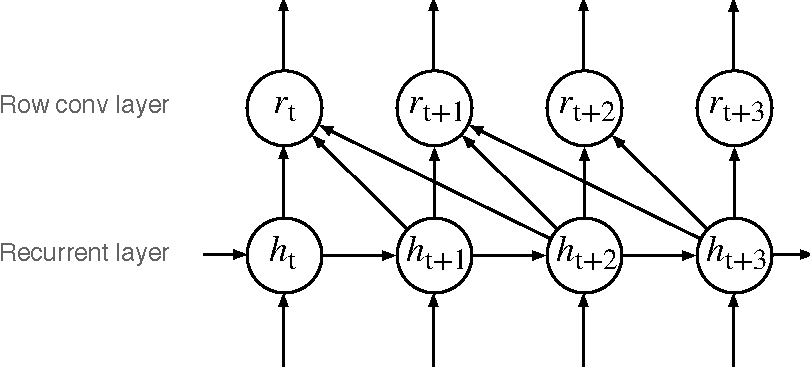
\includegraphics[width=0.6\textwidth]{scaling_asr/figures/row_conv}
\caption{The row convolution architecture with two time-steps of future context.}
\label{fig:scaling_asr:row_conv}
\end{figure}

To accomplish this, we employ a special layer that we call row convolution,
shown in Figure~\ref{fig:scaling_asr:row_conv}. The intuition behind this layer
is that we only need a small portion of future information to make an accurate
prediction at the current time-step. Suppose at time-step $t$, we use a future
context of $\tau$ steps. We now have a feature matrix $h_{t:t+\tau} = [h_t,
h_{t+1}, ..., h_{t+\tau}]$ of size $d\times(\tau+1)$. We define a parameter
matrix $W$ of the same size as $h_{t:t+\tau}$. The activations $r_t$ for the
new layer at time-step $t$ are 

\begin{align}
\label{eq:scaling_asr:rowconv}
r_{t,i} = \sum_{j=1}^{\tau+1} W_{i,j} h_{t+j-1, i}, {\rm \ for\ } 1 \leq i \leq d.
\end{align}

Since the convolution-like operation in Eq.~\ref{eq:scaling_asr:rowconv} is row
oriented for both $W$ and $h_{t:t+\tau}$, we call this layer row convolution.

We place the row convolution layer above all recurrent layers. This has two
advantages. First, this allows us to stream all computation below the row
convolution layer on a finer granularity given little future context is needed.
Second, this results in better CER compared to the best bidirectional model for
Mandarin. We conjecture that the recurrent layers have learned good feature
representations, so the row convolution layer simply gathers the appropriate
information to feed to the classifier. 

%% TODO, decide where to put these results
%Results for a unidirectional Mandarin
%speech system with row convolution and a comparison to a bidirectional model
%are given in Section~\ref{section:deployment} on deployment. 

\subsection{Language Model}
\label{sec:scaling_asr:languagemodel}

We train our RNN Models over millions of unique utterances, which enables the
network to learn a powerful implicit language model. Our best models are quite
adept at spelling, without any external language constraints. Further, in our
development datasets we find many cases where our models can implicitly
disambiguate homophones---for example, ``he expects the Japanese agent
\emph{to} sell it for \emph{two} hundred seventy five thousand dollars''.
Nevertheless, the labeled training data is small compared to the size of
unlabeled text corpora that are available. Thus we find that WER improves when
we supplement our system with a language model trained from external text. 

We use an \emph{n}-gram language model since they scale well to large amounts
of unlabeled text~\cite{hannun2014deepspeech}. For English, our language model
is a Kneser-Ney smoothed 5-gram model with pruning that is trained using the
KenLM toolkit~\cite{heafield2013} on cleaned text from the Common Crawl
Repository\footnote{\url{http://commoncrawl.org}}. The vocabulary is the most
frequently used 400,000 words from 250 million lines of text, which produces a
language model with about 850 million \emph{n}-grams. For Mandarin, the
language model is a Kneser-Ney smoothed character level 5-gram model with
pruning that is trained on an internal text corpus of 8 billion lines of text.
This produces a language model with about 2 billion \emph{n}-grams.

During inference we search for the transcription $y$ that maximizes $Q(y)$
shown in Equation~\ref{eq:scaling_asr:decoding}. This is a linear combination
of $\log$ probabilities from the CTC trained network and language model, along
with a word insertion term~\cite{hannun2014deepspeech}. 

\begin{equation}
\label{eq:scaling_asr:decoding}
Q(y) = \log (p_{\textrm{ctc}}(y|x)) + \alpha \log(p_{\textrm{lm}}(y))  + \beta \: \textrm{word\_count}(y)
\end{equation}

The weight $\alpha$ controls the relative contributions of the language model
and the CTC network. The weight $\beta$ encourages more words in the
transcription. These parameters are tuned on a development set. We use a beam
search to find the optimal transcription~\cite{hannun2014firstpass}.

\begin{table}
\centering
\begin{tabular}{l  l  r r r r r r}
\toprule
Language & Architecture & \multicolumn{3}{c}{Dev no LM} & \multicolumn{3}{c}{Dev LM} \\
\midrule
English  & 5-layer, 1 RNN & & 27.79 & & & 14.39 & \\
English  & 9-layer, 7 RNN & & 14.93 & & & 9.52 & \\
Mandarin & 5-layer, 1 RNN & & 9.80  & & & 7.13 & \\
Mandarin & 9-layer, 7 RNN & & 7.55  & & & 5.81 & \\
\bottomrule
\end{tabular}
\caption{Comparison of WER for English and CER for Mandarin with and without a
         language model.}
\label{table:scaling_asr:languagemodels}
\end{table}

Table~\ref{table:scaling_asr:languagemodels} shows that an external language
model helps both English and Mandarin speech systems. The relative improvement
given by the language model drops from 48\% to 36\% in English and 27\% to 23\%
in Mandarin, as we go from a model with 5 layers and 1 recurrent layer to a
model with 9 layers and 7 recurrent layers. We hypothesize that the network
builds a stronger implicit language model with more recurrent layers. 

The relative performance improvement from a language model is higher in English
than in Mandarin. We attribute this to the fact that a Chinese character
represents a larger block of information than an English character. For
example, if we output directly to syllables or words in English, the model
would make fewer spelling mistakes and the language model would likely help
less.

\subsection{Adaptation to Mandarin}
\label{sec:scaling_asr:chinesemodel}

The techniques that we have described so far can be used to build an end-to-end
Mandarin speech recognition system that outputs Chinese characters directly.
This precludes the need to construct a pronunciation model, which is often a
fairly involved component for porting speech systems to other
languages~\cite{shan2010}. Direct output to characters also precludes the need
to explicitly model language specific pronunciation features. For example we do
not need to model Mandarin tones explicitly, as some speech systems must
do~\cite{shan2010, niu2013}.

The only architectural changes we make to our networks are due to the
characteristics of the Chinese character set. Firstly, the output layer of the
network outputs about 6000 characters, which includes the Roman alphabet, since
hybrid Chinese-English transcripts are common. We incur an out of vocabulary
error at evaluation time if a character is not contained in this set. This is
not a major concern, as our test set has only 0.74\% out of vocab characters.

We use a character level language model in Mandarin as words are not usually
segmented in text. The word insertion term of
Equation~\ref{eq:scaling_asr:decoding} becomes a character insertion term. In
addition, we find that the performance of the beam search during decoding
levels off at a smaller beam size. This allows us to use a beam size of 200
with a negligible degradation in CER. In
Section~\ref{sec:scaling_asr:results_mandarin}, we show that our Mandarin
speech models show roughly the same improvements to architectural changes as
our English speech models.
